% AI-PENTEST -- export z Jira
\documentclass[11pt,a4paper]{article}

\usepackage[slovak]{babel}
\usepackage[T1]{fontenc}
\usepackage[utf8]{inputenc}
\usepackage{newtxtext,newtxmath} % Times New Roman
\usepackage[margin=2.5cm]{geometry}
\usepackage{booktabs}
\usepackage{tabularx}
\usepackage{graphicx}
\usepackage[hidelinks]{hyperref}

\title{Jira -- Web Pentest Harness}
\author{Projekt AI-PENTEST}
\date{}

\begin{document}
\maketitle

\begin{itemize}
  \item Jira: \url{https://tsybulskyi.atlassian.net/jira/software/projects/MIP/boards/1}
  \item Kľúč projektu: \texttt{MIP} (šablóna Scrum)
  \item Šprint: \textbf{Šprint\_1\_týždeň\_5} (1.~11. -- 8.~11.~2026), cieľ: \emph{Pracovná verzia projektu a prehľadového článku}
\end{itemize}

Každý commit v~repozitári obsahuje Jira issue key, napr.\ \texttt{MIP-3 Prehlad tradicnych nastrojov automatizovaneho testovania}. Históriu commitov obsahuje súbor \texttt{../git\_log.txt}.

\section*{Súbory}

\begin{tabularx}{\textwidth}{@{}lX@{}}
\toprule
\textbf{Súbor} & \textbf{Obsah} \\ \midrule
\texttt{ulohy.csv} & zoznam úloh: kľúč, stav, story points, šprint, zodpovedný člen tímu \\
\texttt{backlog.jpg} & snímka backlogu so šprintom \\
\texttt{board.jpg} & snímka boardu (To Do / In Progress / Done) \\ \bottomrule
\end{tabularx}

\section*{Šprint\_1\_týždeň\_5}

\begin{tabularx}{\textwidth}{@{}lXrl@{}}
\toprule
\textbf{Kľúč} & \textbf{Úloha} & \textbf{SP} & \textbf{Zodpovedný} \\ \midrule
MIP-1 & Doplniť bibliografické zdroje o~LLM agentoch a nástrojoch DAST & 2 & Maksym Tomkevych \\
MIP-2 & Rozšíriť úvod: motivácia, cieľ a štruktúra článku & 2 & Andrii Tsybulskyi \\
MIP-3 & Spracovať prehľad tradičných nástrojov automatizovaného testovania & 3 & Kyrylo Bukhanets \\
MIP-4 & Spracovať prehľad prístupov založených na LLM a agentoch & 5 & Artur Toba \\
MIP-5 & Pridať tabuľku porovnania prístupov & 2 & Kyrylo Bukhanets \\
MIP-6 & Rozpracovať metodiku hodnotenia a definovať metriky & 3 & Andrii Tsybulskyi \\
MIP-7 & Rozpracovať kapitolu Diskusia a obmedzenia & 3 & Maksym Tomkevych \\
MIP-8 & Uložiť históriu commitov do git\_log.txt & 1 & Artur Toba \\
MIP-17 & Pridať export Jira do GitHub repozitára & 1 & Andrii Tsybulskyi \\
MIP-18 & Vypracovať formulár VV-A až VV-E & 3 & Andrii Tsybulskyi \\
MIP-19 & Vypracovať formulár VV-F & 5 & Andrii Tsybulskyi \\
MIP-20 & Zosúladiť názov článku so zameraním, primárny zdroj & 1 & Andrii Tsybulskyi \\
MIP-21 & Rozšíriť formulár VV-F na 50--60\,\% rozsahu & 3 & Andrii Tsybulskyi \\
MIP-22 & Pridať PDF prehľadového článku do repozitára & 1 & Andrii Tsybulskyi \\
MIP-23 & Usporiadať štruktúru repozitára a pridať README & 2 & Andrii Tsybulskyi \\
MIP-24 & Písmo Times a README v~LaTeXu & 1 & Andrii Tsybulskyi \\ \bottomrule
\end{tabularx}

\section*{Snímky}

\begin{center}
  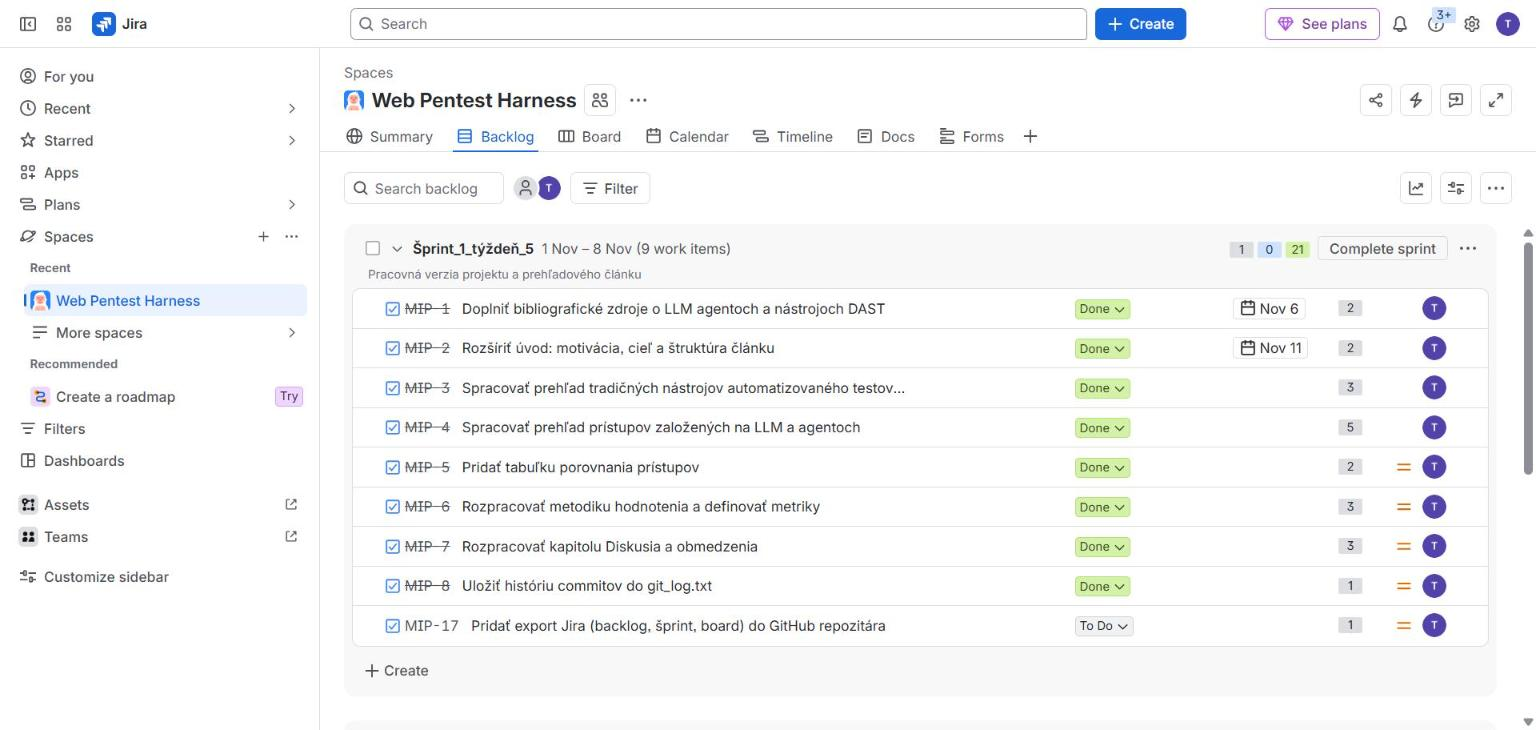
\includegraphics[width=\textwidth]{backlog.jpg}\\[2pt]
  {\small Backlog so šprintom}\\[10pt]
  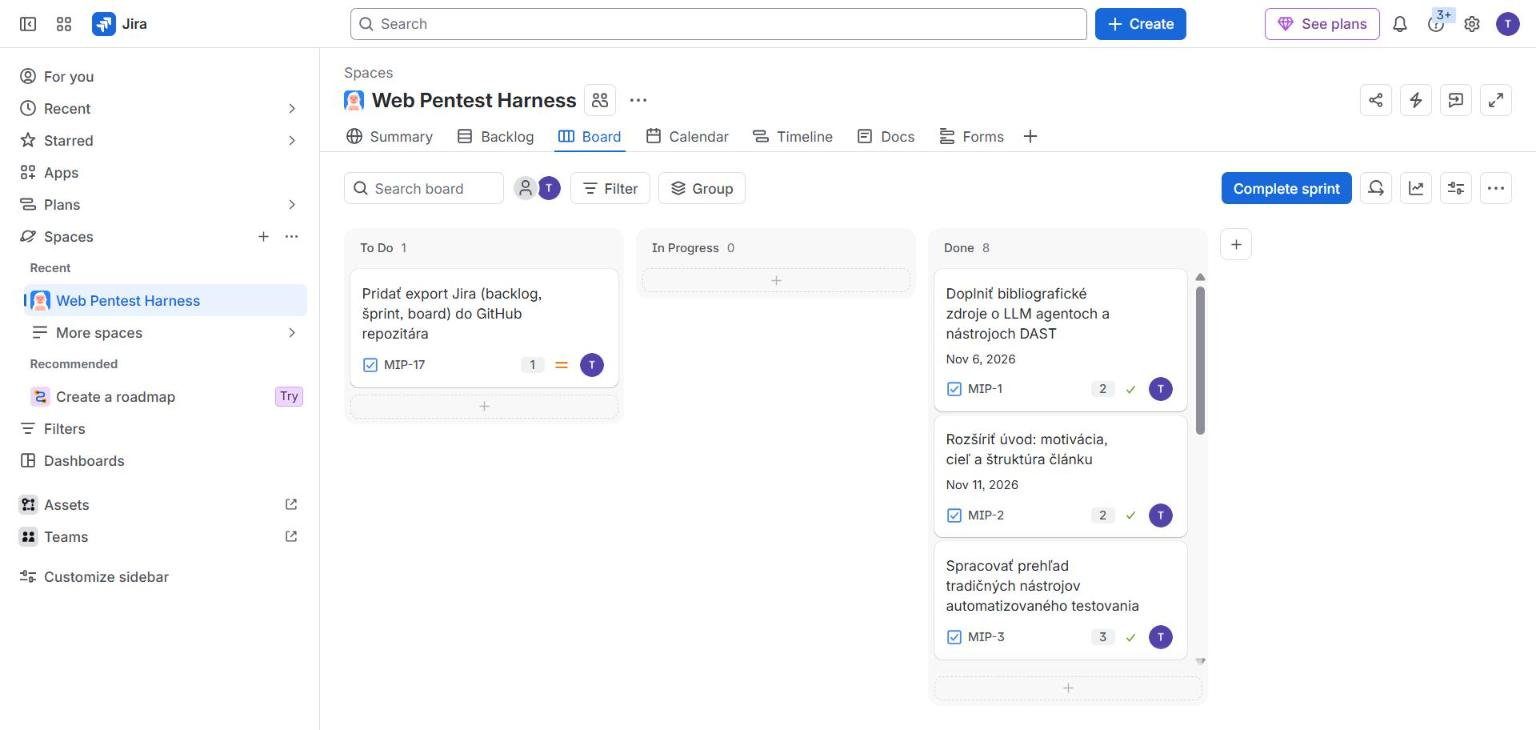
\includegraphics[width=\textwidth]{board.jpg}\\[2pt]
  {\small Board}
\end{center}

\end{document}
